\section{Carbon-Oxygen WD Mergers With Helium Companions}
\label{sec:withhecompanions}

\subsection{Quiet Formation Channels}

Following a merger between a CO WD and an He WD, a heavy CO remnant is formed with a hot He envelope and a fat He disk.  If the disk accretes at near-Eddington or super-Eddington rates, hydrostatic nuclear burning generally results, as the accretion stream will be hot and will not be very dense.  This can be seen from the following argument: from \cite{loreig09} we obtain a disk temperature of approximately $10^7$ K for a 0.3 - 0.5 {\Msun} He-CO merger, and let us assume an accretion rate of 100 {\Msun} yr$^{-1}$.  Using Figs. 1 and 2 from \cite{bild+07} (reproduced here as Fig. \ref{bildstenfig}), we determine that the amount of mass accreted before He ignition will be less than $10^{-3}$ {\Msun}, meaning that $t_{\mathrm{nuclear}} << t_{\mathrm{dynamical}}$, and therefore hydrodynamic burning is never achieved, and the He layer simply expands to accomodate the additional energy generated.

\begin{figure}
\centerline{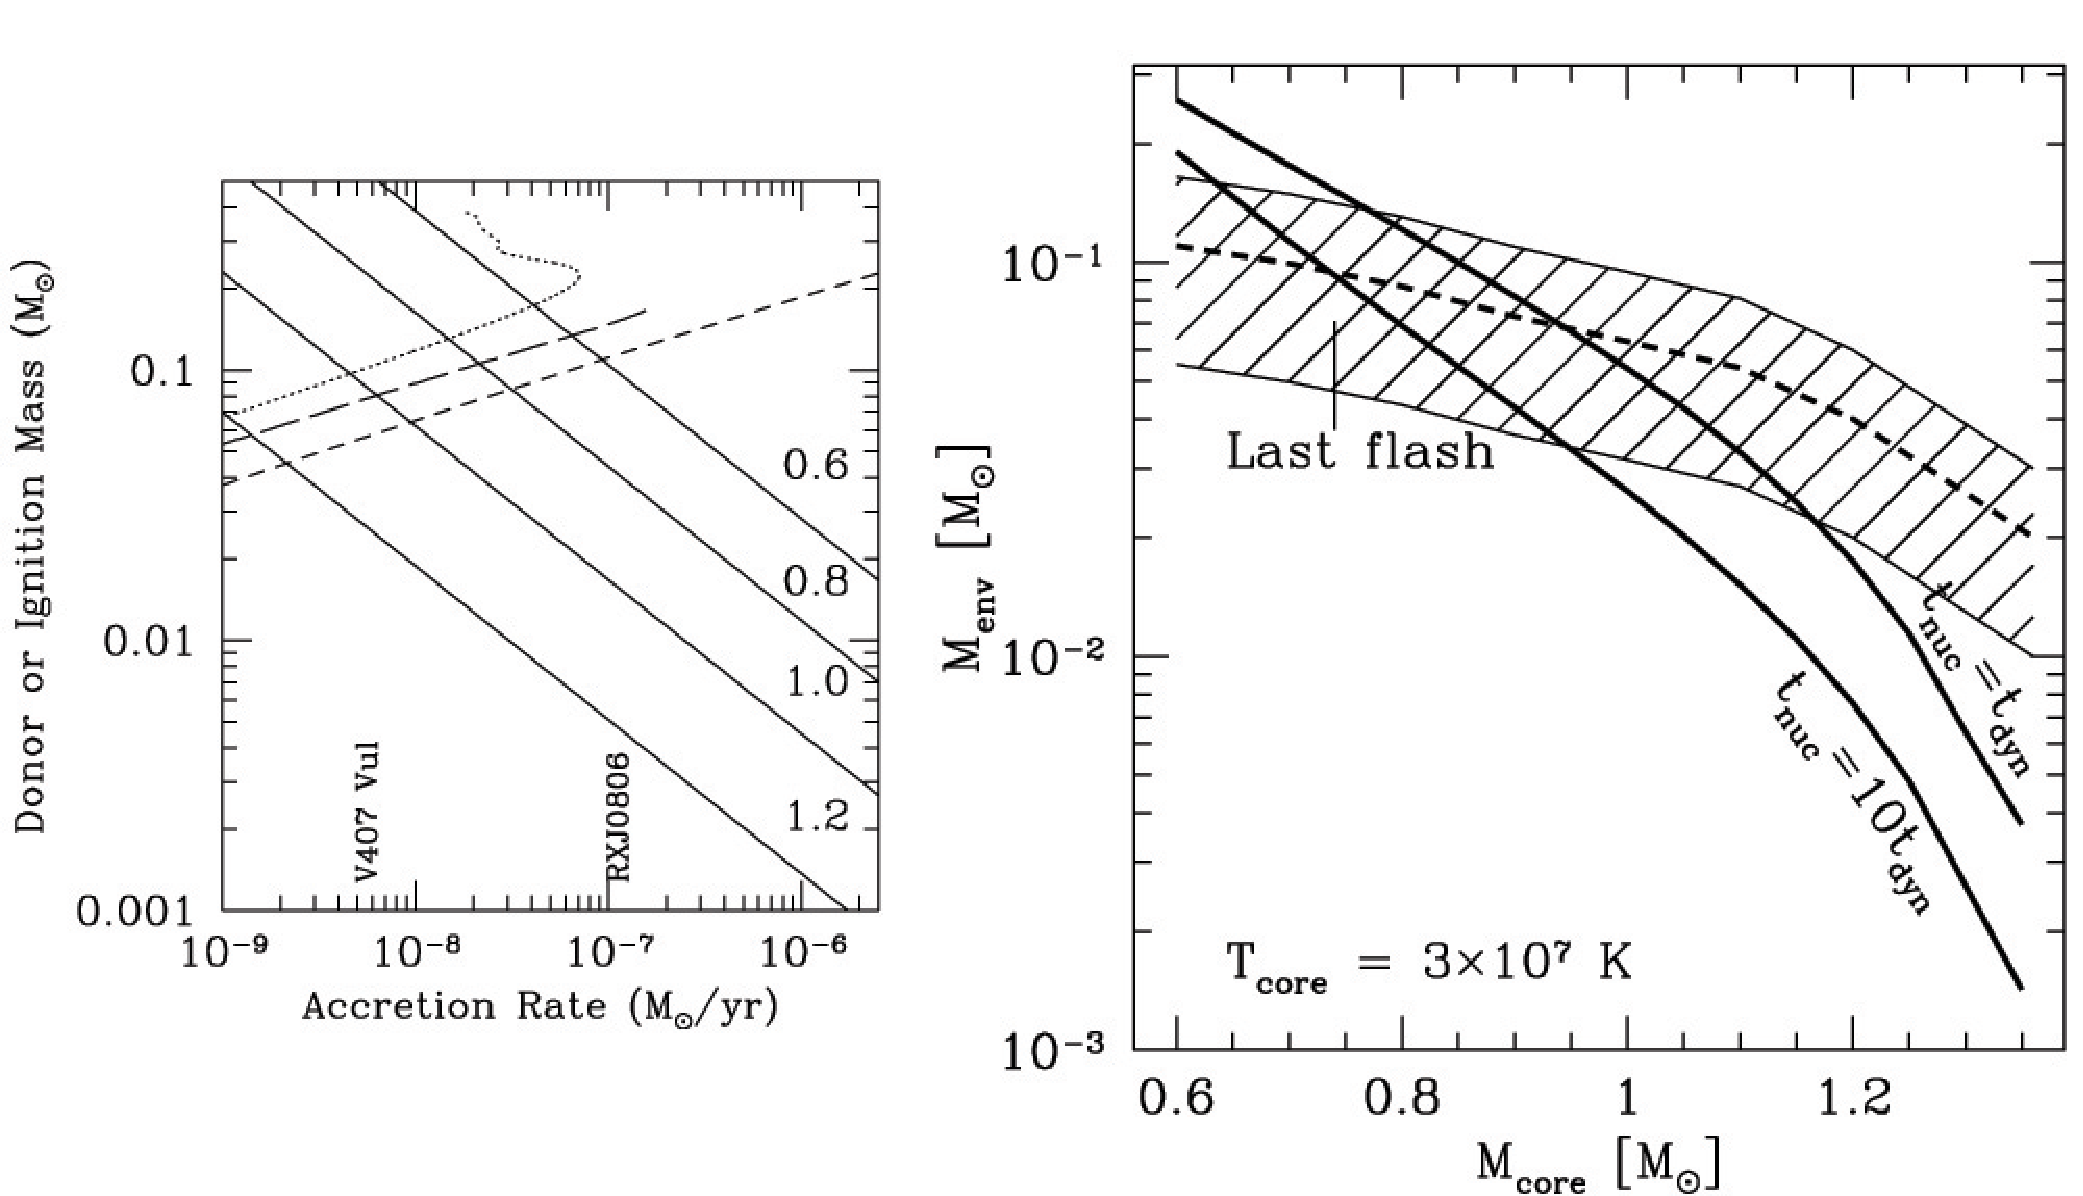
\includegraphics[width=1.0\hsize]{bildstenfig.pdf}}
\caption{Left, estimates (solid lines) for the He ignition mass given accretion of pure He onto a CO WD of 0.6, 0.8, 1 and 1.2 {\Msun}.  The dashed lines represent fully degenerate (short-dashed) and semi-degenerate (long-dashed) He donor mass given a particular accretion rate, and the dotted line represents the same for a He-burning star.  The accretion rate of two particular AM CVn systems is given on the accretion rate axis.  Right, the curves t$_{\mathrm{nuc}}$  = t$_{\mathrm{dyn}}$ and t$_{\mathrm{nuc}}$  = 10t$_{\mathrm{dyn}}$ on a plot of envelope vs. core mass , as well as the approximate regime for the last He flash envelope/core mass relationship for AM CVn stars (dashed line is best estimate, hatched region indicate error).  Anything to the upper right of t$_{\mathrm{nuc}}$  = t$_{\mathrm{dyn}}$ will result in an explosion.  From \cite{bild+07}, their Figs. 1 and 2.}
\label{bildstenfig}
\end{figure}

We therefore expect a number of channels for the remnant of a CO-He merger to continue stellar evolution, rather than explode.  These channels are discussed below.

%Following accretion, the temperature at the base of the atmosphere is dependent upon entropy, which itself is dependent on atmosphere height and accretion rate, both of which are difficult to determine without detailed calculation.

\subsubsection{Extreme Helium, R Coronae Borealis and Hydrogen-Deficient Carbon Star Formation}

\cite{clay+07} semi-analytically calculate disk accretion following a merger between a CO WD of variable mass and an He WD of either 0.2 or 0.4 {\Msun}.  They state that accretion occurs at an average rate of $\sim 30$ - $140$ {\Msun} yr$^{-1}$ (assumed to be steady over time), building up an He atmosphere.   The temperature of the atmosphere, $1$ - $4 \times 10^8$ K, is high enough to ignite He, and significant nuclear processing results (without explosion, in line with Sec. \ref{ssec:mechanicsofwdmergers}) \citep{clay+07}.  \citeauthor{clay+07} suggest that ``hot'' (with nuclear burning) mergers between He WDs and CO WDs will form hydrogen-deficient (HdC) and R Coronae Borealis stars.  This is qualitatively suggested by the extremely low isotopic ratio of $^{16}$O/$^{18}$O $\lesssim 1$ (less than 0.2\% solar), indicating significant production of $^{18}$O.  \citeauthor{clay+07} perform a nucleosynthesis experiment simulating He burning on the merger remnant atmosphere, and recover similar isotopic ratios as are observationally found in RCrB stars.

%\citeauthor{clay+07} suggest that ``hot'' (with nuclear burning) mergers between He WDs and CO WDs will form hydrogen-deficient (HdC) and R Coronae Borealis stars.  This is qualitatively suggested by the extremely low isotopic ratio of $^{16}O/^{18}O \sim 1$ (less than 0.2\% solar), indicating significant production of $^{18}O$.  \citeauthor{clay+07} perform a nucleosynthesis experiment simulating He burning on the merger remnant atmosphere, and obtain an unusually high amount of $^{18}O$ consistent with observations of HdC and RCB stars, and simultaneously obtain high ratios of $^{12}C/^{13}C > 500$, also consistent with these stars \footnote{Interestingly, to obtain the right ratios between multiple isotopes and elements requires the admixture of a thin H envelope from the CO WD \citep{clay+07}.}  The fact that the alternative final helium-flash explanation cannot easily account for observed $^{16}O/^{18}O$ ratios adds weight to the idea that mergers are the progenitors of RCB and HdC stars (though it is not a conclusive argument, as the presence of Li in HdC and RCB stars is not easily explained by mergers) \citep{clay+07}.

\cite{saioj02} also model the post-merger evolution of a remnant formed by a 0.5 - 0.6 {\Msun} CO and a 0.1 - 0.4 {\Msun} He WD, assuming a mass accretion rate of $10^{-5}$ {\Msun} yr$^{-1}$.  Like the He-He merger remnants in \cite{saioj00}, once He burning begins the system evolves toward a yellow giant, during which a series of weak He flashes will occur.  Depending on how much He exists above the shell, the star will remain as a yellow giant for some time, before He exhaustion moves the star toward the blue side of the HR diagram.  The blueward evolutionary track of the giant on a log g vs. log T$_{\mathrm{eff}}$ passes by the values of a number of observed EHes.  Additionally, luminosities, masses, secular evolution and (broadly) surface compositions of observed EHes can be explained by this formation channel.  The rate of CO-He mergers (as given by \cite{nele+01a}) and the time period over which a remnant will appear to be an EHe combined give a of EHes in the Milky Way that roughly matches the observed number.  This suggests that CO-He mergers are the primary progenitor to EHes, and a sizable number of CO-He mergers are quiet.

%\cite{saioj00} note that HdCs and RCrB stars are similar in luminosity and surface composition to EHes (without any nucleosynthesis during the merger), but are cooler, and so they consider their merger model to be equally applicable to HdC and RCrB star formation.  

More recently, \cite{pandl11} concluded that nucleosynthesis is unecessary to explain observed abundances of a large number of elements, including $^{18}$O.  A more detailed analysis by \cite{jeff+11} yielded results that do not give either cold or hot mergers a clear advantage in predicting RCrB and EHe star surface abundances.  It should be noted, however, that simply from merger simulations some nuclear burning is to be expected - these recent results simply show nucleosynthesis may not matter for EHe/RCrB surface composition.

\subsubsection{SdO Star Formation}

Subdwarf B stars will eventually evolve into post-sdB stars, ``hybrid'' CO WDs with thick He envelopes.  Since one significant binary channel for sdB star formation is a common envelope phase between a giant and a WD, there should be a significant number of sdB stars with close-in He WD companions.  \cite{justph11} propose that the merger between the He WD and post-sdB star forms a helium-rich subdwarf O star.  They take their merger to be the standard core and accretion disk, and then perform a slow accretion of the disk onto the core at a sub-Eddington rate with nuclear burning artificially surpressed.  Once the merger is complete, they ignite He fusion, and find that on a log g vs. log T$_{\mathrm{eff}}$ plot the majority of the merger product's life is spent close to the values of observed sdO stars.  An order of magnitude estimate from the formation channel statistics of \cite{han+03} gives similar observed sdO/sdB ratios as is seen in surveys.  Since nuclear burning was not treated in full, it is not obvious if He flashes could occur over the course of the remnant's evolution.

%\subsubsection{DQ WD Formation}

\subsection{Helium Envelope Disruption}
\label{ssec:heliumenvelopedisruption}

As shown above, if accretion rates for the disk onto the merger remnant are above $\sim 10^{-5}$, hydrostatic burning ensues.  If, however, accretion rates are below $\sim 10^{-6}$ {\Msun} yr$^{-1}$, a He thermonuclear explosion could result that disrupts the outer He layer of the star - this can also be seen from Fig. \ref{bildstenfig}.  If this event is a detonation, known as a .Ia supernova, the detonation wave may even travel into the CO core, producing a second, carbon-oxygen, detonation.  Accretion rates are critically dependent on the viscosity of the thick post-merger disk.  Based on estimates from \citeauthor{loreig09} of the viscous timescale, core accretion could as low as $10^{-10}$ - $10^{-14}$ {\Msun} yr$^{-1}$ if the viscosity is laminar, or as high as $10^2$ {\Msun} yr$^{-1}$ if viscosity is turbulent.  If we entertain the possibility of very low viscosity rates, then a He envelope disruption becomes much more likely.

\cite{guil+10} suggests another possible explosion channel.  During the merger itself accretion rates ranging from $10^{-5}$ - $10^{-2}$ {\Msun} yr$^{-1}$ will result in shearing within the accreted He envelope, which then creates large-scale Kelvin-Helmholtz instabilities.  These instabilities form over-dense regions that periodically compress the inner regions of the envelope, possibly resulting in conditions for detonation.  Using the results of SPH simulations, \cite{guil+10} simulate unstable WD binary mass transfer in an adaptive mesh code, and find detonation may be possible on a (0.6 - 0.9 {\Msun}) CO WD that has accreted $~sim$ 0.1 {\Msun} of He.  \citeauthor{guil+10} did not study if this process could also occur during post-merger disk accretion.

\subsubsection{He Novae and Deflagrations}

\cite{woosk10} carry out an extensive investigation into He shell detonations, including the conditions within the He shell necessary for detonation.  An explosion will occur so long as the dynamical timescale is longer than the nuclear timescale.  Whether this explosion is a helium nova, or a deflagration or detonation of the entire shell, depends on the convective timescale compared to the ''runaway timescale''.  \citeauthor{woosk10} define the runaway timescale as the time it takes for He (with its current temperature) to rise to extremely high temperatures if convection were artificially turned off.  From their simulation results, they take $\tau_{\mathrm{run}} \approx 2$ s to be a good trace of the boundary between nova and detonation/deflagration, which they translate to a relationship between density and pressure.  Similarly, to form a detonation shockwave via the Zel'Dovich mechanism requires that the ratio of distance between two points over the difference in their nuclear runaway timescales be larger than the sound speed to create a detonation wave.  This translates to (using the assumption of adiabaticity of the temperature gradient) a relationship between density and temperature, which is plotted alongside simulation results in Fig. \ref{woosleyfig}.  Simulations show that these semi-analytical estimates should be trusted only to first order.

\begin{figure}
\centerline{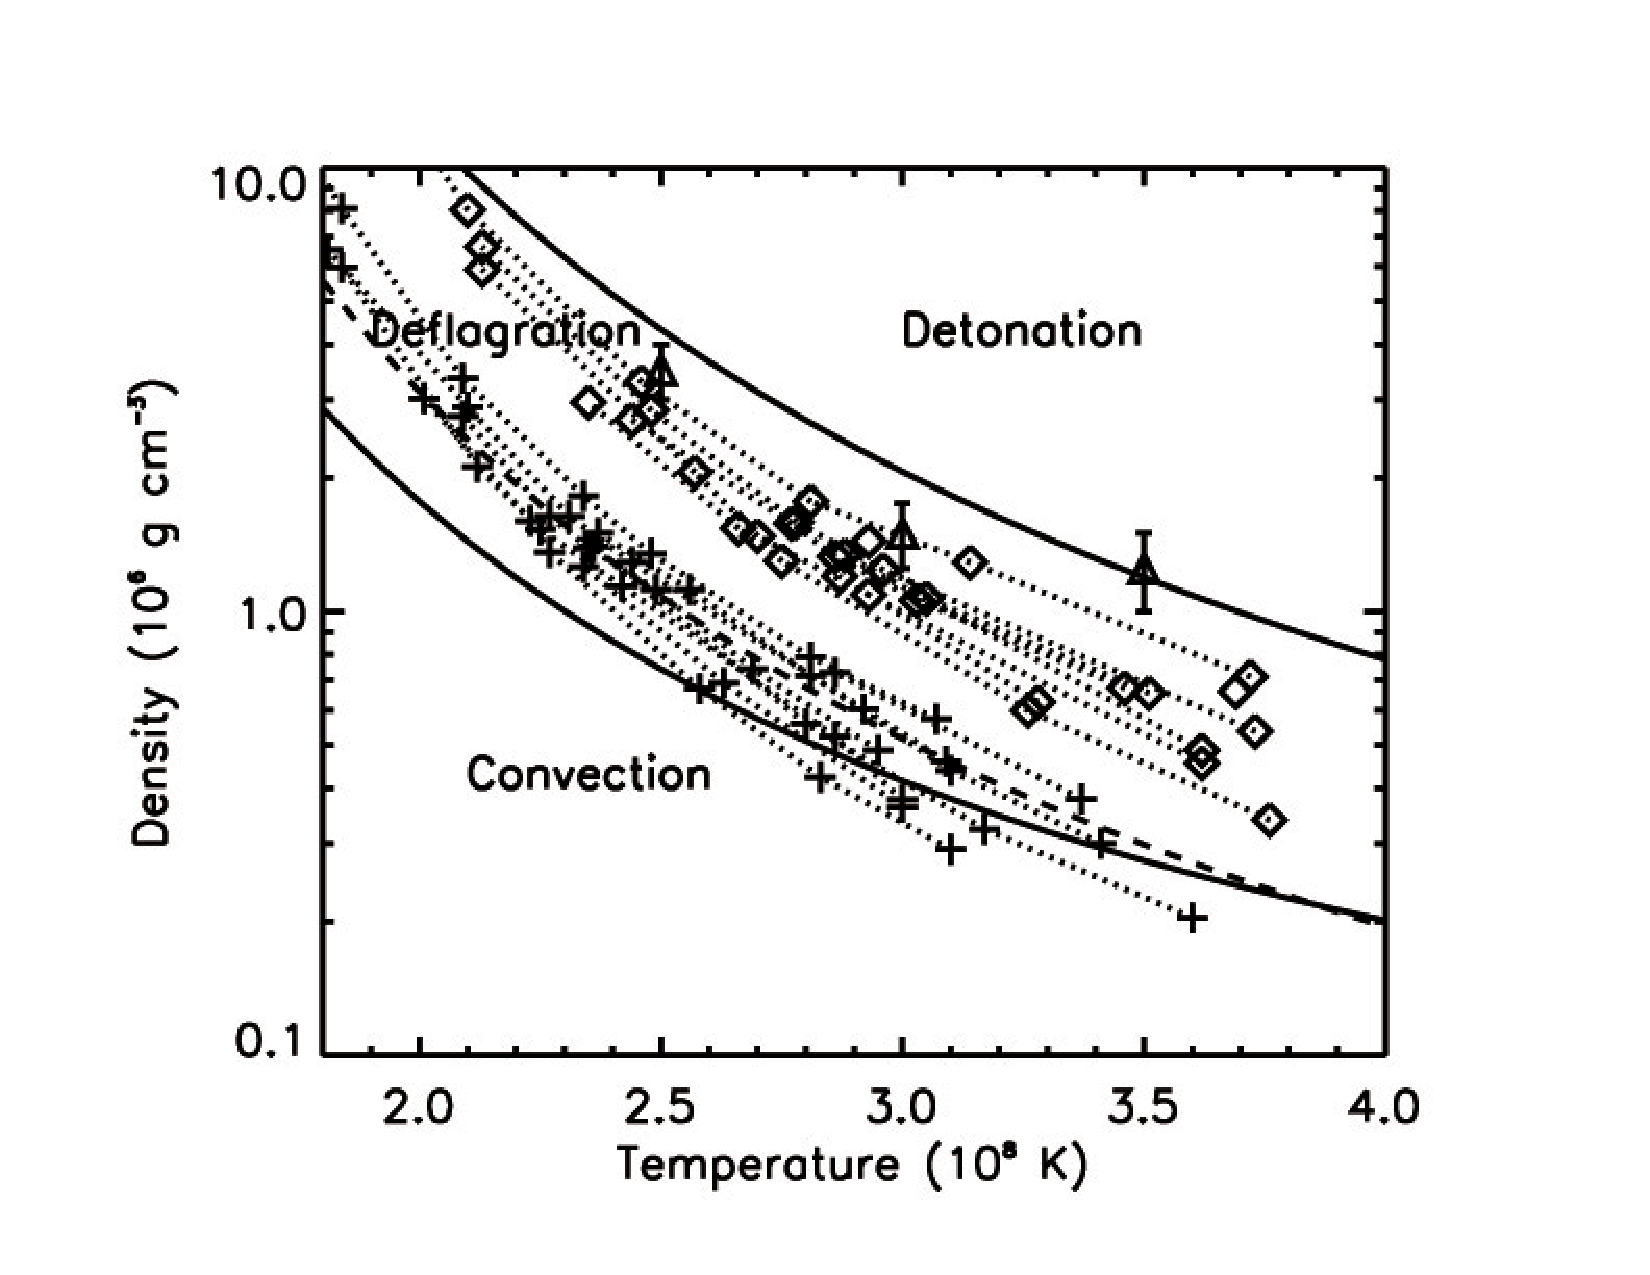
\includegraphics[width=1.0\hsize]{woosleyfig.pdf}}
\caption{A plot of density versus temperature for the He burning region, with the regions for He novae, deflagrations and detonations indicated.  Along with the two analytic estimates of the boundaries of the different regions, a number of simulations are also plotted here.  Diamonds indicate planar (1D) simulations that eventually reach a thin burning shell luminosity of $10^{47}$ erg s$^{-1}$, and crosses indicate simulations that achieve $10^{46}$ erg s$^{-1}$.  Dotted lines connecting diamonds/crosses indicate families of simulations for which the accreting CO WD was identical, but the accretion rate is varied.  All simulations that reached $10^{47}$ erg s$^{-1}$ detonated, and most that reached $10^{46}$ erg s$^{-1}$ deflagrated.  Discrepancy between the analytic estimates and the simulations are due to simulations accounting for gas dynamics and utilizing a more correct equation of state.  Apparently, dividing the analytic deflagration-detonation border by four (arbitrary value) gives a better fit to the simulations (dotted line).  The deflagration-detonation border determined by fine-zone simulations looking single-point detonations are given by triangle points.  From \cite{woosk10}, their Fig 2.}
\label{woosleyfig}
\end{figure}

Below a critical density/temperature given in Fig. \ref{woosleyfig}, convection can effectively carry away energy from the thin shell, resulting in He novae, which are covered in another section of the report.  In the intermediate region between the $\tau_{\mathrm{run}} \approx 2$ condition for explosion and the condition for detonation is the regime for He deflagrations, which are weak (peak B-band magnitude of $\sim$ -15, ejecta velocities of $\sim$ 6000 km s$^{-1}$ for unburned He, and slower for heavier elements), fast-evolving explosions that produce $\sim$ 0.1 {\Msun} of mostly intermediate-mass elements, or IMEs, ($< 10^{-4}$ {\Msun} {\Ni}) and are powered primarily by $^{48}$Cr \citep{woosk10}.  For the two deflagrations simulated by \citeauthor{woosk10}, both ejected most of the accreted He envelope, but processed very little of it.  He deflagrations are covered in another section of the report as well.

Note that some of \cite{wald+10}'s simulations skirt perilously close to the deflagration regime, while \cite{shen+10}'s simulations have initial conditions more firmly in the detonation regime.

\subsubsection{He Detonation Without CO Detonation (.Ia Supernova)}

% THIS IS WRONG: A merger between a {\Msun} CO WD and a lower-mass {\Msun} He WD will result in a cold CO core surrounded by a hot He envelope and disk.  If the disk subsequently accretes onto the remnant core at the prodigeous rates suggested by \citeauthor{clay+07} and \citeauthor{loreig09} (their turbulent viscosity rates), it is conceivable that compressional heating will drive the base of the He core to high enough temperatures and densities to detonate, (see Sec. \label{ssec:withcarbon-oxygencompanions} for a similar argument for CO WDs).  Alternatively, hot-spots created during the merger may reach similar conditions (\textit{a la} \citeauthor{pakm+10}'s CO-CO merger situation) and detonate.

\cite{woosk10}, \cite{shen+10} and \cite{wald+10} all simulate in 1D detonations at the base of the merger remnant He envelope, with CO burning artificially supressed, and all find the detonation unbinds the entire He outer layer of the remnant, while the CO layer is left relatively intact.  Of these, \citeauthor{wald+10} is particularly interesting due to the higher mass ratio between the CO core and He shell (which would more likely for a merger).  \citeauthor{wald+10} explore a range of CO core (0.45 - 0.6 {\Msun}) and He envelope (0.15 - 0.3 {\Msun}) masses and find that, for those detonations on CO cores below 0.6 {\Msun}, explosions produce large quantities of $^{40}$Ca, $^{44}$Ti and $^{48}$Cr, and very little {\Ni}.  For a given CO core mass, the mass fraction in the ejecta of {\Ni} increases with the mass of the He shell.  Additionally, {\Ni} mass fraction can be reduced by polluting the remnant's envelope with CO - at $\sim 10^8$ K, $\alpha$ capture onto carbon is faster than the 3-$\alpha$ process, allowing carbon to effectively slow the nuclear reaction rate of He.  Simulated light curves have a rise time of $\sim$ 7 days, a $\sim$ -11 to -18 peak bolometric magnitude, and highly differing late-time behaviour, depending on the mix of radioactive species produced.

\cite{shen+10} and \cite{woosk10} also simulate He shell detonations in 1D, focusing on detonating thin ($\sim$ 0.02 - 0.1 {\Msun}) He shells on top massive cores (0.6 {\Msun} CO - 1.2 {\Msun} ONeMg) to simulate .Ia SNe.  \citeauthor{shen+10}, however, also simulate detonations of 0.2 - 0.3 {\Msun} envelopes over 0.6 {\Msun} cores, and their resulting light curves and spectra are in general agreement with those of \citeauthor{wald+10}, despite having a different code and a more realistic detonation initialization (though they also do not consider core detonations).  Resulting light curves are, again, highly varied.  As an example, in their 0.6 {\Msun} CO - 0.3 {\Msun} He detonation, 0.3 {\Msun} is ejected (of which 65\% is {\Ni}), with a average asymptotic velocity of $1.3 \times 10^{4}$ km s$^{-1}$ and kinetic energy of $5.3 \times 10^{50}$ erg s$^{-1}$.  The peak bolometric magnitude obtained is -18.  \citeauthor{woosk10} simulates the acutal He accretion process, and provide detailed analysis of the process leading from accretion to explosion.  Their simulations reproduce light curves with a range of peak values and ${\delta}m_{15}$ (number of magnitude drops 15 days after the start of the SN) similar to those found by \citeauthor{shen+10}.  Ejecta velocities and spectroscopic features are also similar between the two papers.  \cite{woosk10} also note that hotter CO WD accretors tend to produce weaker, faster explosions that resemble the He deflagrations mentioned in the previous section.

%\cite{frye+09} simulate a .Ia in an enshrouded environment, and manage to obtain -18 as well, but why do they only get -16 in an un-enshrouded case?

%\cite{woosk01}, \cite{shen+10} and \cite{wald+10} all simulate in 1D detonations at the base of the He envelope of such a remnant, with CO burning artificially supressed\footnote{The CO burning suppression is to prevent spurious centre-lit CO detonations arising from the assumption of spherical symmetry in the detonation shockwaves \citep{wald+10}.}.  They find the detonation unbinds the entire He outer layer of the remnant.  Of these, \citeauthor{wald+10} is interesting in particular due to the higher mass ratio between the CO core and He shell (which would more likely for a merger).  \citeauthor{wald+10} explore a range of CO core (0.45 - 0.6 {\Msun}) and He envelope (0.15 - 0.3 {\Msun}) masses and find that, for those detonations above CO cores below 0.6 {\Msun}, explosions produce large quantities of $^{40}$Ca, $^{44}$Ti and $^{48}$Cr, and very little {\Ni}.  For a given CO core mass, the mass fraction in the ejecta of {\Ni} increases with the mass of the He shell.  Additionally, they note {\Ni} mass fraction can be reduced by polluting the remnant's envelope with CO - at $\sim 10^8$ K, $\alpha$ capture onto carbon is faster than the $\alpha$ process, allowing carbon to effectively slow the nuclear reaction rate of He.  \citeauthor{wald+10}'s simulations suggest that the envelope will be unstable to convection and allow for CO dredge-up, and \citeauthor{loreig09} note appreciable amounts of C and O in the hot envelope of their 0.3 - 0.5 {\Msun} He-CO merger remnant.  Simulated light curves have a rise time of $\sim$ 7 days, a -15 to -18 peak bolometric magnitude, and highly differing late-time behaviour, depending on the mix of radioactive species produced.

%\cite{shen+10} also simulate He shell detonations in 1D, focusing on detonating thin ($\sim$ 0.02 - 0.1) He shells on top massive cores (0.6 CO - 1.2 ONeMg) to simulate .Ia SNe.  They do, however, also simulate detonations of 0.2 - 0.3 {\Msun} envelopes over 0.6 {\Msun} cores, and their resulting light curves and spectra are in general agreement with those of \citeauthor{wald+10}, despite having a different code and a more realistic detonation initialization (though they also do not consider core detonations).  The trend of increasing {\Ni} production with increasing shell mass is reproduced in both simulations, and a 0.6 CO - 0.2 He, the one simulation common to both studies, both simulations produced comparable amounts of unburned $^4He$ and similar nucleosynthetic producs (\citeauthor{wald+10} produced more {\Ni} and less intermediate mass elements).  For their 0.6 {\Msun} CO - 0.3 {\Msun} He detonation, 0.3 {\Msun} is ejected (of which 13\% is {\Ni} and 12\% is $^{44}$Ti), with a average asymptotic velocity of $1.3 \times 10^{4}$ km s$^{-1}$ and kinetic energy of $5.3 \times 10^{50}$ erg s$^{-1}$.  The peak bolometric magnitude obtained is -18.

%We should note that \cite{wald+10}, \cite{shen+10} and \cite{woosk10} all perform simulations detonating thin He shells over massive CO cores in order to simulate .Ia detonations; the resulting explosions also feature significant amounts of intermediate mass elements (the amount goes down as mass goes up), but much less mass is ejected, and in general peak light is much dimmer with a faster rise time.

%THIS IS WRONG \footnote{While \citeauthor{shen+10} having significantly more unburned He than \citeauthor{wald+10} should have an effect on He absorption line strengths, but because neither code accounts for non-local thermal equilibrium (``non-LTE'') effects such as non-thermal electron excitation caused by Compton scattering of $\gamma$ rays (required to explain He absorption lines in Ib SNe), the differences due to unburned He are suppressed.}

%http://texblog.wordpress.com/2007/08/28/placing-figurestables-side-by-side-subfigure/ tells you how to do this without Photoshop.

\begin{figure}
\centerline{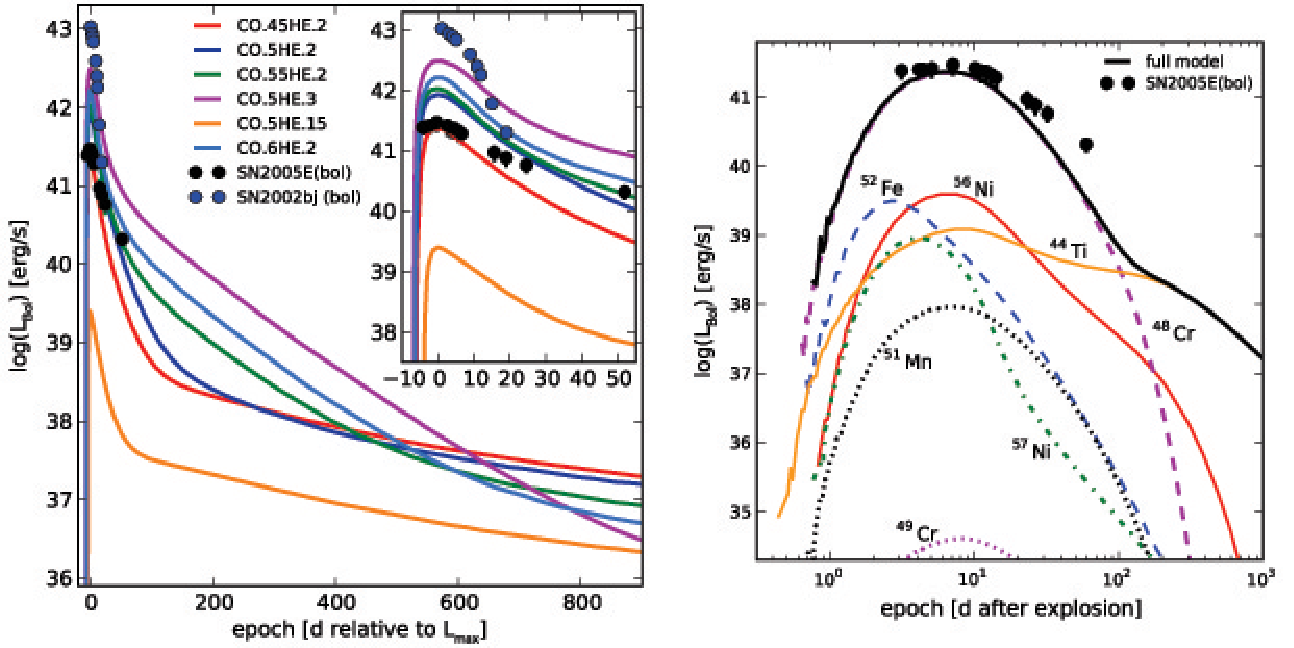
\includegraphics[width=1.0\hsize]{waldmanfigure.pdf}}
\caption{Left: bolometric light curves of 1D explosion models simulated by \citeauthor{wald+10}, compared to type Ib SN 2005E and SN 2002bj.  Error bars of the observed SN include errors due to unobserved bands.  Right: light curve for SN 2005E compared with a 0.45 {\Msun} CO core, 0.2 {\Msun} He envelope remnant (\citeauthor{wald+10}'s best fit to SN 2005E), along with the light curve contributed by each radioactive decay chain.  Note that at early times the light curve is dominated by $^{48}$Cr, and at late times by $^{44}$Ti.}
\label{waldmanfigure}
\end{figure}

He shell detonation has been proposed as an explanation for fast, low-luminosity type Ib SNe that produce very little {\Ni}, have low ejecta masses and have moderate ejecta velocities, and spectroscopically show strong lines of He, Ca and Ti \citep{pere+10a,wald+10}.  The prototype of this class is SN 2005E, which had (assuming only {\Ni}-decay powered light curves) 0.28 {\Msun} of ejecta, 0.003 {\Ni} produced, and $1.1 \times 10^{4}$ km s$^{-1}$ average ejecta velocity \citep{pere+10a}.  While these explosions could be caused by core-collapse of $\sim$ 10 {\Msun} stars, these SNe appear from both young and old stellar populations, and debate is still ongoing regarding the environments that spawn such SNe (Ibs also typically have far greater ejecta masses and greater nucleosynthetic output) \citep{kawa+10,pere+10a,wald+10,pere+11}.  Another class of fast SN, SN 2002bj-like SNe (peak B-band light $\sim -18.5$, 0.15 {\Msun} ejected - most of it {\Ni}, on order $10^{50}$ ergs kinetic energy), has also been proposed to be caused by He shell detonations due to their correlation with older stellar populations and their low ejecta masses \citep{pere+10b}. For SN 2002bj, however, the evidence for He in the spectrum is less conclusive than for SN 2005E \citep{pere+10b, pozn+10}.

\citeauthor{wald+10} compared their models to the light curve of SN 2002bj, and light curve and spectrum of SN 2005E.  While they cannot exactly reproduce the light curve and spectrum of SN 2005E, their 0.45 CO - 0.2 He detonation model can reproduce SN 2005E's peak-light (-15th mag) and ejecta velocities.  On the other hand, the models have faster late-time declines, and faster evolving spectra, than SN 2005E. Though most observed features are replicated by the light curve, their strengths are not.  Both facts suggest that SN 2005E had a somewhat different total ejecta mass (the model gives $\sim$ 0.2 {\Msun}; an estimate from observations assuming a light curve powered only by {\Ni} gives $\sim$ 0.28 {\Msun}) and composition.  SN 2002bj-type light curves are either too bright at peak light, or decay too quickly, to fit well to the curves of either \citeauthor{wald+10} or \cite{sim+10}, suggesting either alternative explosion mechanisms or the need for a more detailed study of He shell detonation parameter space.

\cite{brow+11} study a sample of 12 extreme low mass (ELM; $\leq 0.25$ {\Msun}) He WDs, 11 of which are in binary systems \footnote{\citeauthor{brow+11} make the case that the 12th is likely a pole-on binary system, since low mass He WDs cannot be made through single-star evolution}.  From this sample they determine the combined merger and stable mass transfer system creation rate to be $4 \times 10^{-5}$ yr$^{-1}$ (which they note is likely an underestimate), of which they estimate, by using Eqn. \ref{qcrit2}, that $\sim 30$\% of this rate will be He-CO WD mergers, meaning the He-CO WD merger rate is $\sim 1 \times 10^{-5}$ yr$^{-1}$.  Supplementary material from \citeauthor{pere+10a} give the rate of calcium-rich SNe to be $\sim 7$\% of the total SN Ia rate, which \citeauthor{brow+11} give as $5 \times 10^{-3}$, meaning that mergers between low mass He and CO WDs only accounts for a fraction of calcium-rich SNe.  Other progenitors may include mergers involving heavier He WDs (much more common, cf. Secs. \ref{ssec:populationstatistics} and \ref{ssec:possibleexplosivenuclearburning}), He transfer from non-WD companions, or other detonation mechanisms \footnote{Including mergers of ELM He WDs with other HE WDs would approximately double \citeauthor{brow+11}'s rates.}.


% Such mergers then contribute $\sim 10$\% of the total estimated rate of underluminous SNe, $\sim 1 \times 10^{-4}$ yr$^{-1}$ \citep{fole+09,brow+11}.  Note, however, that this last value is based on single event statistic

%Note that the total rates \citeauthor{brow+11} give include .Ia from AM CVn systems formed from ELM WD colaescences.  Since this is not a useful number to cite for

%A nuclear detonation of an He shell around a CO core will have a distinct signature (WHAT IS IT?).  Such events have been cited as being responsible for low-mass, low-to-normal luminosity and fast-evolving SNe.

%Kawabata thinks it comes from a 10 {\Msun} star (2010Natur.465..326K), though a mapping of the region finds no evidence of recent star formation or a younger stellar population that could explain the origin of a 10 {\Msun} star 2011ApJ...728L..36P.

\subsubsection{He Detonation With CO Detonation}

If a detonation were to occur in He, it is possible for this detonation to propagate into the CO core as a edge-lit (i.e. CO-He interface-lit) CO detonation, disrupting the entire WD.  An outward propagating He detonation could also, via inward propagating shockwaves, compress the CO core to the point at which its centre ignites.  An He detonation triggering a CO detonation is known as the ``double-detonation'' scenario, and has been well-studied (cf. references in \cite{woosk10}, \cite{finkhr07} and \cite{fink+10}).  \citeauthor{woosk10} find very little difference in outcome between edge-lit and compressional double-detonations.

A significant issue discussed by \citeauthor{woosk10} is that for a compressional detonation the inward shocks must converge in a region less than 100 km across to light the CO detonation.  Current 1D simulations artificially satisfy this convergence, but if an He detonation is to be reached the He nuclear runaway layer must fragment into small sections that do not communicate with each other, and whether a simultaneous detonation at multiple points is possible is still an open question.  A probable outcome is an asynchronous detonation of several extended regions in the runaway layer, and the resulting lack of shockwave convergence makes a CO detonation more difficult \citep{woosk10}.  An issue for the edge-lit detonation is propagation of the He detonation wave into CO core, which is a function of density, altitude of the He detonation from the CO core, and the degree of He-CO mixing at the interface between the two layers.  \citeauthor{woosk10} note that both problems require a more detailed understanding, and treatment in 3D simulations.

\cite{finkhr07} perform 2D simulations (z-axis vs. radius coordinates) of compressional detonations from various initial flame geometries, such as single point detonations, spherical shell detonations, and single/multiple torus detonations.  Their initial system consists of either a 0.8 {\Msun} CO core with a 0.2 {\Msun} He shell, or a  0.9 {\Msun} core with a 0.1 {\Msun} shell.  They also followed up a single point detonation using a full 3D cartesian simulation.  They find that the majority of their detonations result in a secondary core explosion, and they argue that due maximum density being resolution limited, it is likely all their simulations should lead to explosions if their resolution was infinite\footnote{This is due to the fact that \citeauthor{finkhr07} find that all of their initial flame geometries eventually produce inward propagating shocks that are roughly spherically symmetric.}.  Their explosions are comparable to (though somewhat weaker than) normal SNe Ia: all 1.0 {\Msun} are ejected, with an average speed of $\sim 10^4$ km s$^{-1}$, and $\sim$ 0.4 {\Msun} {\Ni} is produced.  Their 3D result is very similar to their 2D results, only producing 0.05 {\Msun} more {\Ni}.  Follow-up work (still in 2D) was presented in \cite{fink+10} with a refined nuclear reaction chain.  The results from \cite{finkhr07} still hold, except that more of the He shell burned into IMEs during the explosion rather than {\Ni}, which would help make the explosion look more like an SN Ia (see below).  Again the entire star is ejected, about 0.2 - 1.1 {\Msun} of {\Ni} is produced (highly dependent on progenitor mass) and 10$^{51}$ ergs asymptotic energy is released.  These results has been challenged by \citeauthor{woosk10}, who state that \citeauthor{fink+10} uses a completely convective envelope, while their simulations of comparable initial masses, using more correct initial conditions where convection is frozen-out, burn He all the way to {\Ni}.  Note that \cite{finkhr07} and \cite{fink+10} use perfect mirror symmetry and assume complete burning from He to Ni during explosions, both somewhat unrealistic assumptions that significantly increase the chances of detonation \citep{guil+10}.

Traditionally double-detonations have been contenders for SN Ia progenitors.  Model spectra from such events, however, do not match spectra of observed SN Ia - IME lines are too weak in the models, owing to the nuclear processing of the outer He layer to {\Ni} \citep{woosk10,finkhr07,vkercj10,howe10}.  Still, one supernova, the over-luminous SN 1991T, did have large amounts of {\Ni} in its outer layers, and may have been a double-detonation \citep{finkhr07}.  Centre-lit CO detonations without any He envelope have recently been shown by \cite{sim+10} to look much like SNe Ia, which suggests that if a very thin envelope were to start a double detonation the resulting SN would more closely resemble an SN Ia \citep{howe10}. \citeauthor{woosk10} set an upper limit to the mass of the envelope at $\sim 0.05$ {\Msun}.  Both \citeauthor{woosk10} and \citeauthor{fink+10} showed that detonating shell masses lower than this value may still cause a double-detonation.

It is interesting to note that if double detonations produce explosions that do not look like SN Ia, we should see a significant fraction of SN with similar brightnesses to SN Ia, but with differing spectroscopic features.  That we do not see this either means that double-detonations do not work as we understand them, all double-detonations are of the thin-envelope variety, or the conditions for reaching detonation are not often created during slow accretion of He onto CO WDs.

\section{Carbon-Oxygen WD Mergers With Carbon-Oxygen Companions}
\label{sec:withcarbon-oxygencompanions}

\subsection{ONeMg WD Formation}

Rapid accretion of the remnant disk onto the core following a CO-CO merger may result in off-centre carbon ignition, which forms a carbon burning shell.  The energy released during nuclear burning is either emitted as neutrinos, or retained by the WD and conducted inward from the shell \citep{saion98}.  Therefore the shell propagate inwards, turning the remnant into an ONeMg WD over a timescale of $10^{3}$ - $10^{4}$ yr \citep{yoonpr07,saion98}.  \citeauthor{saion98} simulate the evolution of the burning shell assuming an accretion rate of $1 \times 10^{-5}$ {\Msun} yr$^{-1}$, and find no explosive phenomenon.  Once an ONeMg WD is formed, an accretion-induced collapse (AIC) is generally thought to follow if the WD is too massive or if accretion continues \citep{yoonpr07,saion98}.  AICs are described in Sec. \ref{sec:onemg}.

\subsection{Type Ia Supernovae from CO-CO Mergers}

The most spectacular transient that could potentially come of a CO WD merger is undoubtedly a type Ia supernova (SN Ia).  The ight curves of SNe Ia and the physical processes that can be discerned from them is a well-studied subject, and will not be covered here in detail.  In general for SN Ia, the total ejecta mass is the mass of the progenitor WD or WD binary, $\sim$ 0.4 - 0.7 {\Msun} of {\Ni} is produced, and $\sim 10^{51}$ ergs of energy is released \citep{blin+06}.  Excellent review articles on the subject that do go into much more detail include \cite{howe10} and \cite{hilln00}.

The canonical progenitor of an SN Ia, however, is a CO WD accreting mass stably from a non-degenerate companion (rather than another CO WD) \citep{hilln00,howe10}.  As the Chandrasekhar mass {\Mchan} is approached, temperatures and pressures near the core of the CO WD exceed what is required to ignite carbon fusion, and a runaway nuclear process results \citep{hilln00,howe10}.  This picture has several shortcomings.  It firstly requires physical fine-tuning: a precise accretion rate during stable mass transfer is required to prevent recurring novae or stable AGB-like nuclear shell burning (neither of which lead to a massive explosion) \citep{vkercj10,howe10}.  Binaries that accrete at the correct rate should emit low-energy X-rays, and the number of such ``super-soft'' X-rays sources observed in the universe is far outweighed by the number needed to account for the observed SN Ia rate \citep{vkercj10,howe10}.  If an {\Mchan} WD were to experience nuclear runaway, an ad-hoc deflagration-to-detonation transition is needed in order to obtain ejecta velocities and compositions consistent with observed SNe Ia \citep{hilln00,howe10}.  This suggests considering double-degenerate mergers as a channel for creating SNe Ia.

%Lastly, it is difficult to explain outlier SN Ia light curves, particularly ones that appear to have super-{\Mchan} ejecta masses (unless spherical symmetry is broken) \citep{taubenberger}.  Though this might be fixed using asymmetry arguments and off-centre detonations.

\subsubsection{Chandrasekhar Mass CO Detonations}

The Chandrasekhar double-degenerate merger picture is one where, following the merger, disk accretion drives the core to the Chandrasekhar mass, generating an explosion.  One issue that has plagued this model is achieving {\Mchan} without igniting off-centre carbon burning, which leads to an ONeMg WD \citep{yoonpr07,loreig09}.  As noted earlier in Sec. \ref{ssec:heliumenvelopedisruption}, accretion is critically dependent on the timescale for viscous transfer of angular momentum between the disk and core, and as a result could range from as low as $10^{-11} - 10^{-14}$ to as high as $10^2$ {\Msun} yr$^{-1}$ \citep{loreig09}.  \citeauthor{yoonpr07} perform a very detailed investigation of a 0.6-0.9 {\Mchan} CO-CO merger remnant evolution, and determined that if the rate of angular momentum loss (to the disk or via gravitationl radiation) is slow enough that neutrino cooling can balance heating from loss of rotational support, and if $\dot{M}_\mathrm{acc} \lesssim 5 \times 10^{-6}$ - $10^{-5}$ {\Msun}/yr, an {\Mchan} core may be created.  It may also be possible, from variations in the angular momentum loss timescale, to ignite carbon fusion at masses slightly above or below {\Mchan}, giving variation to SN Ia explosion strengths.  Note that the resulting star must still trigger a deflagration-to-detonation transition.

If the deflagration-to-detonation occurs off-centre, an asymmetric ejecta composition results.  \cite{sim+07} study how light curves are affected by this asymmetry using a toy explosion and radiative transfer model, and find that, in their most extreme asymmetric models, peak light can vary by as much as $\sim$ 1.5 mag while time to peak light may vary by $\sim$ 8 days.  This variation is due to the fact that there there is more material enshrouding the {\Ni} on one side of the star.  \cite{sim+07} note that such SNe Ia are likely to be rare, as if they were common the tight correlation between explosion bolometric flux vs. recession velocity would have much more noise.  This effect is then likely confined to a peak light variation of $\sim$ 0.5 mag and rise time variation of $\sim$ 3 days, making asymmetry a second-order effect.  Asymmetry in SNe Ia is also a well-studied topic (cf. for example references in and to \cite{sim+07}).

\cite{frye+10} model in 1D the detonation of an {\Mchan} WD surrounded by envelopes of various masses and compositions of either CO or He.  Such a situation would be expected for a merger, and not for a single-degenerate  or stable-mass transfer system (since the secondary would not surround the primary).  They find (see Fig. \ref{fryerfig}) that enshrouding delays, compared to normal SN Ia, UV emission from the initial outburst, and shock heating (generally ignored in SN Ia simulation) further enhances and broadens the UV light curve, sometimes even creating a double-peaked curve.  V-band emission is also significantly broadened compared to normal SN Ia.  There are also early spectral differences between the models and observed SNe Ia.  \citeauthor{frye+10} conclude that such enshrouded systems should not produce ordinary SNe Ia, and suggest that merger rates of different massed WDs may conspire to make it so that the majority of merger CO WD binaries barely exceed {\Mchan}, minimizing the effects they see in their simulations.  Also, notably, a few SNe Ia, such as SN 2002ic and SN 2005gj do appear to have been Ia inside extended envelopes (another section of this report suggests a different interpretation of these SNe).

\begin{figure}
\centerline{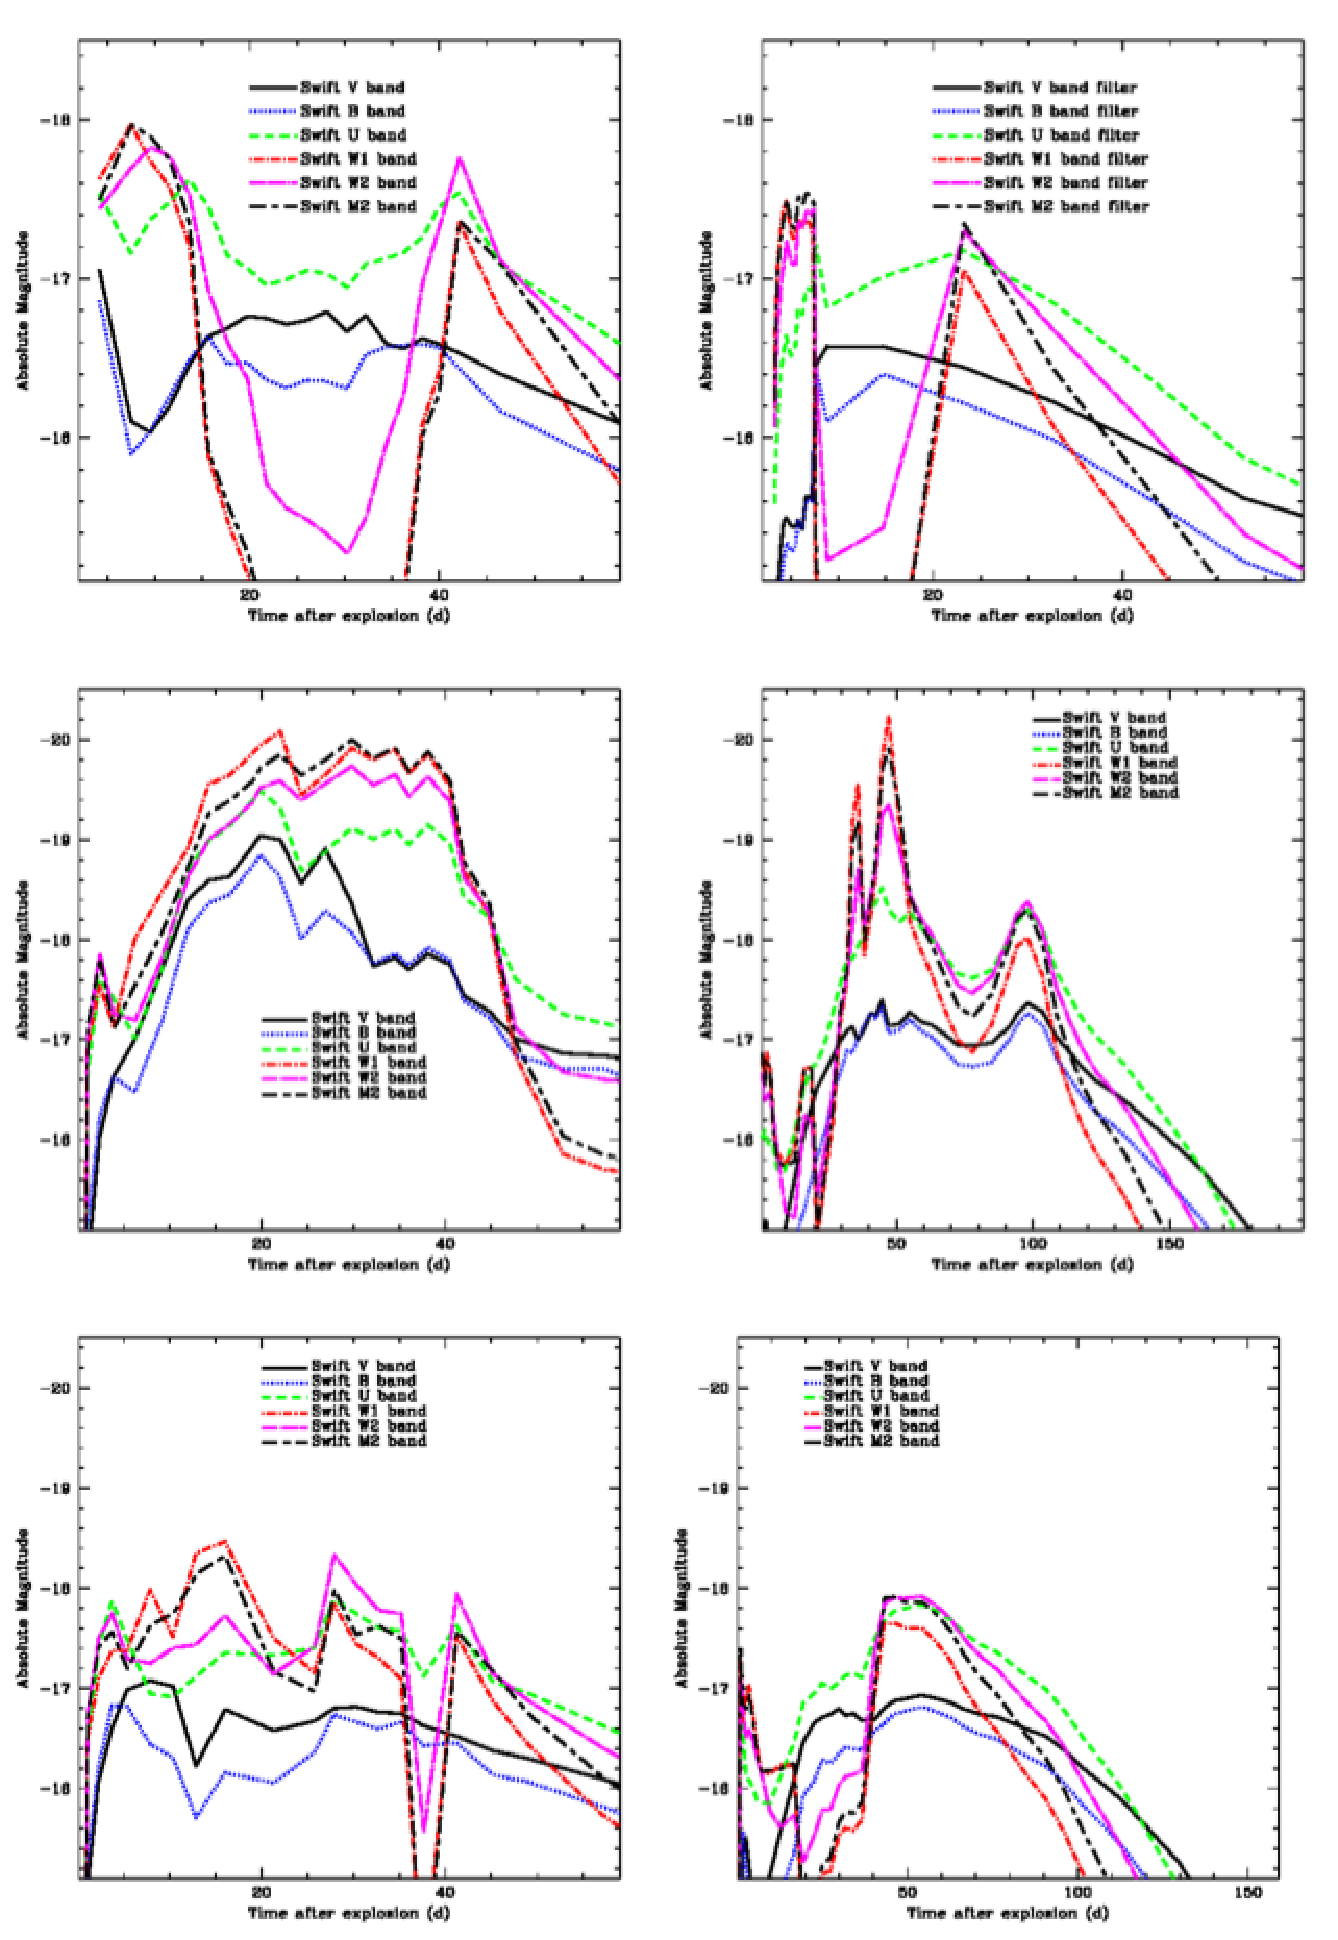
\includegraphics[width=0.8\hsize]{fryerfig.pdf}}
\caption{Simulated light curves of enshrouded SNe Ia with differing extended envelope masses and compositions, for a number of \textit{Swift} visual and UV bands.  All the plots on the left column are for He envelopes, and the right for CO envelopes; the envelope masses are 0.1 (top column), 0.35 and 0.7 {\Msun}.  Note that in a number of plots the U, W and M bands appear to have either a plateau of emission or a double peak.  From \cite{frye+10}, their Fig. 9.}
\label{fryerfig}
\end{figure}

A detonation carries its own signature distinct from the canonical SN Ia light curve.  \cite{pirocw10} calculate that the shockwave from a detonation breaking out from the surface layers of the WD should create a $10^{-2}$ s burst of hard X-rays with peak luminosity $\sim 10^{44}$ erg s$^{-1}$, followed by a cooling tail.  Peak absolute magnitude in the V band is around -9 to -10, and occurs one day after the detonation.  \citeauthor{pirocw10} add that the visibility of this transient will depend on the WD radius at the time of the detonation, and {\Ni} decay soon after the explosion.  \cite{hofls09} suggests the X-ray burst energy peak luminosity is closer to $10^{48}$ - $10^{50}$ erg s$^{-1}$, though these numbers may drop to the level of \citeauthor{pirocw10} if expansion and adiabatic cooling over the diffusion time are taken into account.  \citeauthor{frye+10} study shock breakout in an enshrouded SN Ia and find that the X-ray emission (like the UV emission described above) is delayed and spread out over a longer period of time, and the peak luminosity decreases, as the mass of the envelope surrounding the Ia increases.  They note, however, that the mass distribution is at least as important as the amout of mass, and therefore using shock breakout to determine whether the SN Ia is enshrouded requires further investigation.

%-http://adsabs.harvard.edu/abs/2011arXiv1103.3062C
%-http://adsabs.harvard.edu/abs/2007A%26A...465L..17H
%-http://adsabs.harvard.edu/abs/2007ApJ...660.1344R

If the two WD masses are nearly the same, a different SN Ia channel emerges.  \cite{pakm+10} simulate the merger of two 0.89 CO WDs, and track points of high temperature and density near the core of the star.  Finding a point with density $3.8 \times 10^6$ g cm$^{-3}$ and temperature $2.9 \times 10^9$ K, they transfer the remnant model onto a grid-based hydrodynamic code and artificially detonate the point.  The result is a sub-luminous, low-velocity explosion with a peak B-band magnitude of $\sim -17$ following  a rise time of around 15 days, asymptotic kinetic energy of $1.3 \times 10^{51}$ ergs, and 1.8 {\Msun} of ejecta, with 0.1 {\Msun} of that being \Ni.  They also note incomplete silicon burning over a large fraction of the WD leads to well-mixed iron and silicon group elements, which is not seen in the layered ejecta of ordinary SNe Ia.  \citeauthor{pakm+10} compare their results to 1991bg-like underluminous SNe Ia, and find both light curves and spectra to be in very good agreement.  They also use a population synthesis model to determine that such mergers should account for 2-11\% of SNe Ia, which is in range of the fraction of observed SNe Ia that are 1991bg-like, regardless of whether normal SNe are created by the single or double-degenerate Chandrasekhar channels.  Follow-up work \citep{pakm+11} shows that the equal mass condition for a detonation could be relaxed to q = $\sim$0.8, although unequal mass mergers should have higher {\Ni} yields (see Sec. \ref{sssec:sub-chandrasekharmasscodetonations}) and hotspots produced are off-centre.  Note this picture is significantly different than the Chandrasekhar model discussed above - the detonation occurs during the merger itself, and not during the accretion phase afterward.  See Fig. \ref{pakmorfigure} for details.

\begin{figure}
\centerline{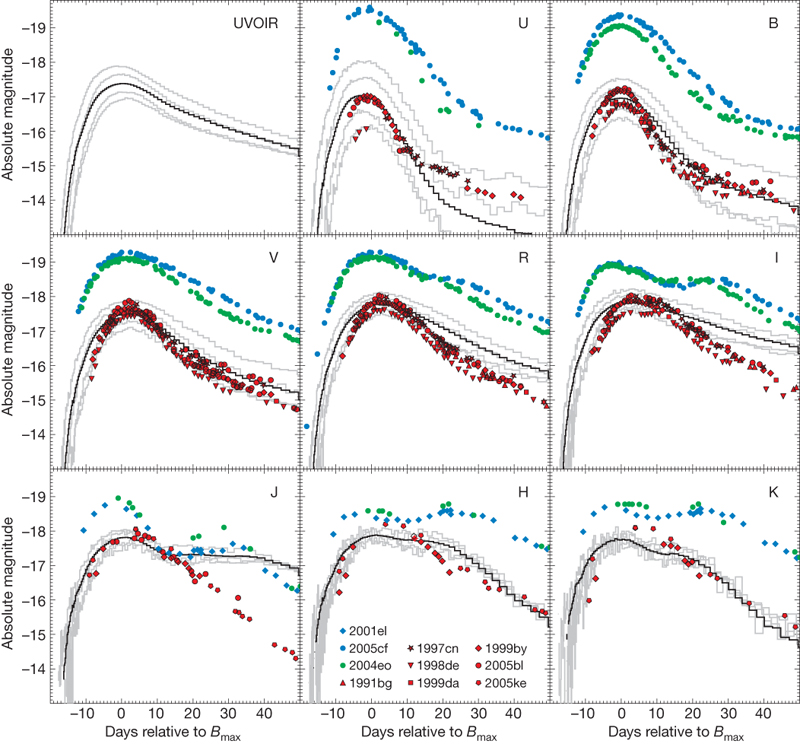
\includegraphics[width=0.8\hsize]{pakmorfig.jpg}}
\caption{Comparison of synthetic light curves from a simulated double-degenerate merger SN Ia with a number of observed 1991bg-like SNe Ia curves.  As the detonation is not spherically symmetric, the shape of the curve depends on viewing angle, and four solid grey curves have been plotted to indicate the distribution of light curves arising from this asymmetry.  The solid black curve is the angle-averaged light curve.  Blue points represent observed light curves for ordinary SNe Ia 2001el, 2005cf and 2004eo, while red points indicate light curves for 1991bg-like SNe Ia.  T = 0 is set to the B-band maximum.  Note that normal supernovae have a secondary maximum in the near-IR, which is not reproduced by either observed 1991bg-like SNe Ia or the synthetic curve.  The synthetic curve does not drop as quickly as observed light curves in the optical and near-IR following peak light.  From \cite{pakm+10}, their Fig. 2.}
\label{pakmorfigure}
\end{figure}

\subsubsection{Sub-Chandrasekhar Mass CO Detonations}
\label{sssec:sub-chandrasekharmasscodetonations}

On the other hand, the majority of CO-CO WD mergers will result in sub-Chandrasekhar mass remnants with hotspots too cold to ignite runaway carbon fusion \citep{vkercj10,loreig09}.  As noted earlier, the remant disk could accrete onto the core in a matter of hours.  \citeauthor{vkercj10} argue that if accretion were so quick, compressional heating would be high enough to create the conditions for carbon fusion at the centre of the remnant core, resulting in a detonation.  This sub-Chandrasekhar picture has the advantage of not reqiring a deflagration-to-detonation transition, and conveniently explains why SN Ia peak luminosity decreases with increasing progenitor age.  Moreover, surveys and population synthesis show the rate of SN Ia from single and double degenerate Chandrasekhar channels combined is less than half the observed SN Ia rate, while the total rate of CO-CO WD mergers regardless of total mass is more than the SNe Ia rate \citep{vkercj10,sim+10}.  The lack of an He envelope negates the ejecta stratification problem that has historically plagued double-detonation models \citep{vkercj10,howe10,sim+10}.  See Fig. \ref{simfig}.

\begin{figure}
\centerline{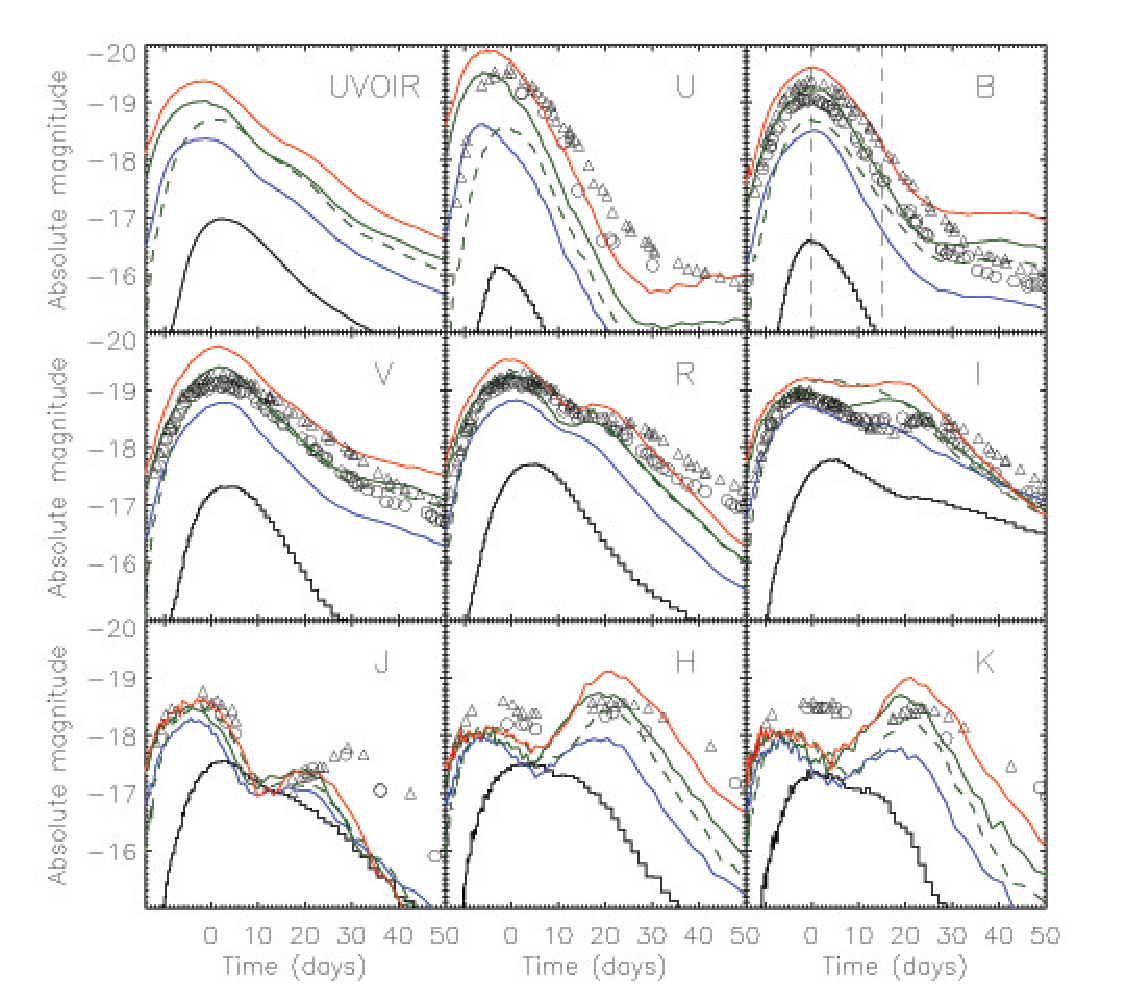
\includegraphics[width=0.8\hsize]{simfig.pdf}}
\caption{Comparison of synthetic light curves from simulated centre-lit detonations in M = 1.15, 1.06, 1.06 (polluted with Ne), 0.97 and 0.88 {\Msun} CO WDs (red, solid green, dashed green, blue and black, respectively) and observed light curves of SN 2004eo and SN 2005cf (circles and triangles, respectively).  Curves tend to drop too quickly after peak light, though \cite{sim+10} note this may be due to how radiative transfer is treated.  Traditionally the sub-Chandrasekhar picture involves the merger of a CO WD and an He WD, which is described in Sec. \ref{sec:withhecompanions}.  These models, having no He envelope, differ from previous models that show {\Ni} stratification that does not agree with observation.  From \cite{sim+10}, their Fig. 2.}
\label{simfig}
\end{figure}

One might expect that since \citeauthor{pakm+10}'s 0.9-0.9 CO WD merger only produced 0.1 {\Msun} of {\Ni}, the detonation of even lighter remnants would be very faint, but {\Ni} production is a strong function of remnant central density.  An equal-mass 0.9-0.9 {\Msun} merger remnant is significantly less dense near its core than a 0.9-0.8 remnant, which means that mergers of unequal mass binaries will generally result in more luminous explosions than equal-mass binaries of the same total mass \citep{pakm+11,vkercj10}.

This picture relies critically on hot-spots being near the centre of the remnant core, and on accretion being on the timescale of hours, and therefore it is an open question how much fine-tuning is required for it to work.

\subsection{Other Types of Explosions}

As is obvious from above, the parameter space of all CO-CO mergers is significantly larger than the space of those mergers that create SNe Ia.  Even if sub-Chandrasekhar mass mergers cannot lead to canonical SNe Ia, they should also still lead to transients of some sort \citep{pakm+10}.

\subsubsection{Pure Deflagration of a Chandrasekhar Mass CO WD}

%NTS: so here's how DTD works: you have a deflagration - this doesn't produce a lot of peak iron, and spreads throughout the whole star.  You then detonate, creating lots of peak iron, but the outer layers of the WD have already expanded due to deflagration, so not much iron is produced there by the detonation.  The whole thing expands more quickly since the detonation releases more energy, and you get a stratification - outer layers strong in Si, inner in Ni.  A pure deflagration, no surprise, has well mixed Ni and Si since the whole thing should look like SN Ia outer layers.

If for some reason a deflagration-detonation transition does not occur, a pure deflagration could result.  \cite{blin+06} model a pure deflagration starting at the centre of a {\Mchan} WD.  The flame propagates outward, generating turbulence that increases the flame propagation velocity.  This runaway process eventually consumes and disruptes the entire star.  \citeauthor{blin+06} show that a pure deflagration produces around 0.2 to 0.4 {\Msun} of {\Ni}, as well as 0.35 to 0.65 $\times 10^{50}$ ergs of KE.  Peak light in B-band is about -18 to -19 mag, and the rise time is $\sim$ 17 days.  {\Ni} is well mixed with IMEs, and there is an excess of unburned material travelling at low velocities.  Variation in nickel and energy produced is due to differing central densities and chemical compositions of the WD progenitors.  \citeauthor{blin+06} find that while synthetic UBV light curves match well with weak SNe Ia that produce below 0.4 {\Ni}, the near-IR has too slow a rise time and does not drop quickly enough following peak light (leading to the bolometric light curve evolving too slowly compared with observations), while the U-band has too fast a rise time and drops too quickly.  Additionally, the near-IR curves lack secondary maxima after peak light that are normally seen in observed SNe Ia \citep{blin+06,phil+07}.  \citeauthor{blin+06} state their models has known shortcomings, and that more refined deflagration models may result in more stratification of ejecta and faster moving ejecta, which should help resolve many of these issues.

Due to the low kinetic energies and amounts of {\Ni} in the ejecta of a pure deflagration, they are contenders for producing SN 2002cx-like supernovae.  These underluminous supenovae have low expansion velocities, no secondary maximum in the light curve, and significantly mixed ejecta, all consistent with pure deflagrations \citep{phil+07}.  \cite{phil+07} compare one of \cite{blin+06}'s models to the light curve of SN 2002cx-like supernova SN 2005hk, and obtain reasonably good fitting, except for a small delay in peak light, and deviation from observation in the IR, and in other bands at late times.  They believe refinements in radiative tranfer codes and fine-tuning of the initial conditions can lead to better fits\footnote{Deflagrations should have strong OI and CI forbidden lines due to an excess of low-velocity unburned material; this is not seen in SN 2002cx-like SN, though higher resolution deflagration simulations appear to reduce the descrepancy \citep{phil+07}.}.  It should be noted that some SNe Ia, such as SN 2008ha, are too underluminous to be described by pure deflagrations.  \cite{fole+09} show that SN 2008ha had a peak luminosity of $\sim 10^{41}$ ergs, a kinetic energy of $2 \times 10^{48}$ ergs, an ejecta velocity of 2000 km $s^{-1}$ and an ejected mass of 0.15 {\Msun} of matter, $4 \times 10^{-3}$ {\Msun} of which was {\Ni}.  This is far too little kinetic energy and mass to be a deflagration \citep{fole+09}.

If the pure deflagration is highly asymmetric (i.e. the entire star explodes but is burned to {\Ni} largely on only one side), then asymmetry effects appear.  \cite{sim+07} simulate a pure deflagration creating 0.448 {\Msun} {\Ni} with such an asymmetry, and find peak magnitude variations of $\sim$ 0.5 mag.

\subsubsection{Failed Deflagrations}

Failed deflagrations of Chandrasekhar mass WDs can also occur.  \cite{cald+04} and \cite{livnah05} both find that for a single off-centre ignition point, the resulting hot ash bubble formed rises very quickly to the surface of the WD, leaving most of the star unburned.  Surface velocities for the hot bubble range from $\sim$ 5000 to $\sim$ 10000 km s$^{-1}$.  From \cite{cald+04}, about 2\% of the star is burned to iron peak elements (about twice as much is burned to IMEs), and only 0.2\% of the star actually reaches escape velocity.  This highly asymmetric explosion, if it managed to eject more material, would be consistent with the properties of SN 2008ha \citep{fole+09}.  (SN 2008ha is also potentially consistent with a transient caused by an AIC; see Sec. \ref{sec:onemg}.)

%Note, I'm ASSUMING 0.075 solar masses is burned, and 0.026 solar masses is iron.


%FUN QUESTION: IF A WD LOST MASS, WOULD IT COOL?

%\citeauthor{loreig09} state that how a CO WD merger remnant may detonate crucially depends on accretion rates, which depend on viscous transfer of angular momentum.  The viscous timescale for laminar viscosity is on the order of $10^{11}$ s, while the turbulent viscous timescale is on order $10^{-4}$ s; therefore, accretion can either be $10^{-12}$ {\Msun}/yr, or $10^{2}$ {\Msun}/yr.  The critical rate of accretion to result in central carbon ignition is $10^{-6}$ {\Msun}/yr: larger values will tend to ignite carbon off-centre, resulting in the creation of an ONeMg WD (CITE SOMEONE), while low accretion values can bring the WD to {\Mchan}, allowing for a centre-lit explosion.

%SEE REF IN YOON, 2ND PARAGRAPH.
